\section{V4}
\subsection{Bias und Präzision}
Die Verzerrung, auch Bias oder systematischer Fehler genannt, ist in der Schätztheorie eine Kennzahl oder Eigenschaft eines Punktschätzers. Die Verzerrung bildet das Gegenstück zur Erwartungstreue und formalisiert, dass ein Schätzer im Mittel von dem zu schätzenden Wert abweicht.
Bias und Präzision sind unabhängig voneinander.
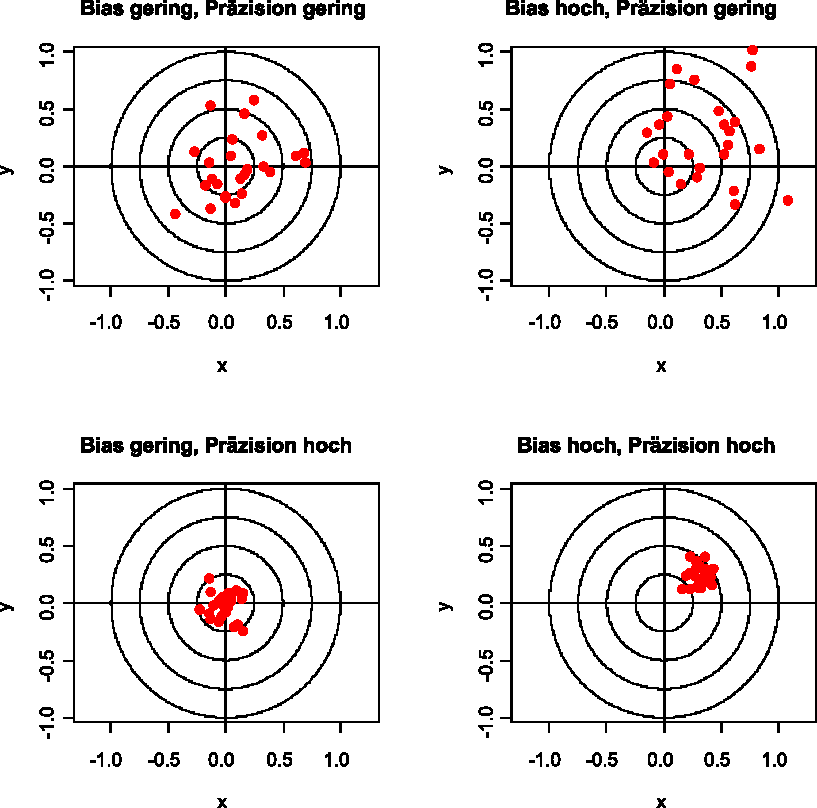
\includegraphics[width=0.5\textwidth]{lectures/V4/pix/bias_precision.pdf}
\begin{itemize}
    \item Zufällige Fehlerwerte sind bedauerlich, aber handhabbar
    \item Selektive Fehlerwerte führen zu Bias!
\end{itemize}

\subsection{Frequentistischer und Bayesianischer Wahrscheinlichkeitsbegriff}
\begin{description}
    \item[Frequentistisch] ~
        \begin{itemize}
            \item Wahrscheinlichkeit eines Ereignisses interpretiert als relative Häufigkeit, mit der es in einer großen Anzahl gleicher, wiederholter, voneinander unabhängiger Zufallsexperimente auftritt
            \item Wahrscheinlichkeit eines einzelnen Ereignisses ist nicht definiert
            \item Beispiele: Münzwurf, Würfeln, Dauer einer Schwangerschaft
        \end{itemize}
    \item[Bayesianisch] ~
        \begin{itemize}
            \item Wahrscheinlichkeit definiert als ``Grad vernünftiger Erwartung'' oder ``Rationale quantifizierung von Unsicherheit'' (z.B. faire Wetten)
            \item Beispiele: Jede Art von Vorhersage (z.B. Regen)
        \end{itemize}
\end{description}

\subsection{Zufallsvariablen (Erwartungswert, Varianz, Standardabweichung, Covarianz, Unabhängigkeit, Randverteilung)}
Zuordnung einer Zahl zu einem Ereignis $A_i$: 

$X: \Omega \rightarrow \mathbb{R}$

\subsubsection{Wahrscheinlichkeitsverteilung einer Zufallsvariablen}
\paragraph{Diskret}
\begin{description}
    \item[Wahrscheinlichkeitsfunktion] (Einzelwahrscheinlichkeit) \\
    $ p(x_i) = P\{X=x_i\} = a_i ~~ (i=1,2,\dots) $
    \item[Verteilungsfunktion] ~\\
    $ F(x)= P\{X \leqslant x \} = \sum_{x_i \leqslant x} p(x_i) $
\end{description}
\paragraph{Stetig}
\begin{description}
    \item[Wahrscheinlichkeitsfunktion] (Einzelwahrscheinlichkeit) \\
    $ p(x) = P\{ X = x \} = 0 ~~ \forall x $
    \item[Verteilungsfunktion] ~\\
    $ F(x)= P\{X \leqslant x \} = \int_{-\infty}^x f(\xi)d\xi $
    \item[Dichtefunktion] (Wahrscheinlichkeitsdichte)\\
    $ f(x) = {d \over dx} F(x) $
\end{description}

\subsubsection{Erwartungswert einer Zufallsvariablen}
\paragraph{Diskret}
$ E[X] = \sum_{i} x_i p(x_i) $
\paragraph{Stetig}
$ E[X] = \int_{-\infty}^{+\infty} x f(x)dx $

\subsubsection{Varianz einer Zufallsvariablen}
\paragraph{Diskret}
$ Var[X] = E[(X-E[X])^2] = \sum_i (x_i - E[X])^2 p(x_i) $
\paragraph{Stetig}
$ Var[X] = E[(X-E[X])^2] = \int_{-\infty}^{+\infty} (x-E[X])^2 f(x)dx $ \\\\
Es gilt: $ E[(X-E[X])^2] = E[X^2] - E[X]^2 $

\subsubsection{Standardabweichung einer Zufallsvariablen}
$ SD[X] = \sqrt{Var[X]} $

\subsubsection{Unabhängigkeit}
Man nennt zwei Ereignisse A und B unabhängig, wenn gilt: \\
$ P\{ A \cap B \} = P\{ A \} \cdot P\{ B \} $. \\
Umformuliert für Zufallsvariablen: \\
Wenn für alle Paare $(x,y)$ gilt: \\
$ F_{XY}(x,y) = F_X(x) \cdot F_Y(y) $, \\
so nennt man die Zufallsvariablen X und Y unabhängig. Im stetigen Fall gilt außerdem: \\
$ f_{XY}(x,y) = f_X(x) \cdot f_Y(y) $

\subsubsection{Kovarianz zweier Zufallsvariablen}
$ Cov[X,Y] = E[(X-E[X])(Y-E[Y])] = E[XY] - E[X]E[Y] $ \\
Man nennt X und Y unkorreliert, wenn $ Cov[X,Y] = 0 $ \\
Korrelationskoeffizient nach Pearson: $ r = {Cov[X,Y] \over SD[X] \cdot SD[Y]} $ \\
Es gilt: X,Y unabhängig $\Rightarrow$ X,Y unkorreliert \\
Aber \textbf{nicht} andersherum!

\subsection{Bedingte Wahrscheinlichkeit, Bayes'sche Lernformel}
\subsubsection{Bedingte Wahrscheinlichkeit}
$ P\{ A|B \} = { P\{ A ~ und ~ B \} \over P\{ B \}} $, $ P\{ B \} > 0 $
\paragraph{Diskret}
$ p_{X|Y}(x|y) = { p_{XY}(x,y) \over p_Y(y)} $
\paragraph{Stetig}
$ f_{X|Y}(x|y) = { f_{XY}(x,y) \over f_Y(y)} $ \\\\
Bei Unabhängigkeit von $X$ und $Y$ gilt $ P(X|Y) = P(X) $.

\subsubsection{Gesetz der totalen Wahrscheinlichkeit}
$ P\{ A \} = \sum_{i=1}^n P \{ A|B_i \}P\{ B_i \} $, für $ \Omega = \bigcup_{i=1}^n B_i $ und $ B_i \cap B_j = \emptyset $, $ i \neq j $

\subsubsection{Satz von Bayes}
$ P\{ B_i | A \} = {P(A|B_i) P(B_i) \over \sum_{j=1}^n P\{ A | B_j \} P\{ B_j \} } $, $ i \neq j $, für $ \Omega = \bigcup_{j=1}^n B_j $ und $ B_i \cap B_j = \emptyset $, $ i \neq j $

\subsubsection{Bayesianische Lernformel}
\begin{description}
 \item[Bayesianisches Lernen:] Vorannahmen mit Unsicherheit (Vorläufige Parameter \textendash{} Prior) $\rightarrow$ Zusätzliche Daten $\rightarrow$ Neue Bewertung der Situation (Revidierte Parameter \textendash{} Posterior)
\end{description}

Seien $ H_1, \dots, H_k $ eine Menge von Hypothesen (z.B. Parameterannahmen zu einem Zufallsexperiment). Seien $D$ beobachtete Daten. Seien $ pr(H_i) $, $ i=1, \dots, k $, die Prior-Wahrscheinlichkeiten für $H_i$ bevor man die Daten erhoben hat. Dann gilt: \\\\
$ \overbrace{P(H_i|D)}^{Posterior-Wk.} = { \overbrace{P(D|H_i)}^{Likelihood ~ unter ~ H_i} \overbrace{P(H_i)}^{Prior-Wk.} \over \underbrace{\sum_j P(D|H_j) P(H_j)}_{Normalisierung}} $

\subsection{Einige wichtige Verteilungsfunktionen}

\subsubsection{Bernoulli-Verteilung}
$ P(X=1) = p $ \\
$ P(X=0) = 1-p $ \\
$ E(X) = p $ \\
$ Var(X) = p(1-p) $

\subsubsection{Binomialverteilung}
$ X \sim Binom(N,p) $, falls $ X= \sum_{i=1}^N Y_i $ und $Y_i \sim Bernoulli(p)$ und unabhängig \\
$ P(X=k) = \binom{N}{k} p^k (1-p)^{N-k} $ \\
$ E(X) = Np $ \\
$ Var(X) = Np(1-p) $

\subsubsection{Normalverteilung}
$ X \sim N(\mu,\sigma^2) $ \\
Dichte: $ f_X(x) = { 1 \over \sqrt{2 \pi \sigma} } exp(-{(x - \mu)^2 \over 2 \sigma^2}) $ \\\\
$ E(X) = \mu $ \\
$ Var(X) = \sigma^2 $\\\\
$ X \sim N(\mu,\sigma^2) \Leftrightarrow {X - \mu \over \sigma} \sim N(0,1) $
\begin{description}
    \item[Zentraler Grenzwertsatz:] Wird eine Größe durch viele kleine additive zufällige Einflüsse beeinflusst, so ist diese häufig normalverteilt
    \item[Beispiele:] Körpergröße, Geburtsgewicht normal verlaufender Schwangerschaften
    \item[3$\sigma$-Regel]
        Sei $ X \sim N(\mu_x, \sigma_x^2) $, dann:
        \begin{itemize}
            \item $ P(X \in [\mu_x - \sigma_x, \mu_x + \sigma_x]) \approx {2 \over 3} $
            \item $ P(X \in [\mu_x - 2 \sigma_x, \mu_x + 2 \sigma_x]) \approx 0.95 $
            \item $ P(X \in [\mu_x - 3 \sigma_x, \mu_x + 3 \sigma_x]) \approx 0.99 $
        \end{itemize}
\end{description}

\subsubsection{Log-Normalverteilung}
Eine Zufallsvariable heißt Lognormalverteilt, wenn ihr Logarithmus normalverteilt ist.
$ f(x) = { 1 \over \sqrt{2 \pi \sigma x} } exp(-{(ln(x) - \mu)^2 \over 2 \sigma^2}) $
\begin{description}
    \item[Analog zur Normalverteilung:] Wird eine Größe durch viele multiplikative zufällige Einflüsse beeinflusst, so ist diese häufig log-normalverteilt
    \item[Beispiele:] Viele Laborwerte, Blutparameter, Genexpression
\end{description}

\subsubsection{Chi\textsuperscript{2}-Verteilung}
Die Summe von N unabhängigen quadrierten standardnormalverteilten Zufallsvariablen ist $ \chi^2 $-verteilt mit N Freiheitsgraden. \\
$ \chi^2 \sim Z_1^2 + \dots + Z_n^2 $ mit $ Z_k \sim N(0,1) $
\begin{itemize}
    \item Wie bei der Normalverteilung ist die Summe unabhängiger Chiquadrat-Verteilungen wieder Chiquadrat-verteilt
    \item Für große N ist die Wurzel Chiquadrat-verteilter Zufallsgrößen normalverteilt
    \item Die Prüfgröße einiger wichtiger statistischer Tests ist Chiquadrat-verteilt
\end{itemize}

\subsection{Aufgaben zur Übung 4}
